%
% File coling2020.tex
%
% Contact: feiliu@cs.ucf.edu & liang.huang.sh@gmail.com
%% Based on the style files for COLING-2018, which were, in turn,
%% Based on the style files for COLING-2016, which were, in turn,
%% Based on the style files for COLING-2014, which were, in turn,
%% Based on the style files for ACL-2014, which were, in turn,
%% Based on the style files for ACL-2013, which were, in turn,
%% Based on the style files for ACL-2012, which were, in turn,
%% based on the style files for ACL-2011, which were, in turn, 
%% based on the style files for ACL-2010, which were, in turn, 
%% based on the style files for ACL-IJCNLP-2009, which were, in turn,
%% based on the style files for EACL-2009 and IJCNLP-2008...

%% Based on the style files for EACL 2006 by 
%%e.agirre@ehu.es or Sergi.Balari@uab.es
%% and that of ACL 08 by Joakim Nivre and Noah Smith

\documentclass[11pt]{article}
\usepackage{coling2020}
\usepackage{times}
\usepackage{amsmath,amsfonts,amssymb}
\usepackage{url}
\usepackage{latexsym}
\usepackage{hyperref}
\usepackage[noabbrev,capitalize]{cleveref}
\usepackage{graphicx}
\usepackage{subcaption}
\usepackage{pgfplots}


\newcommand\jp[1]{(\textbf{JP:} #1)}
\newcommand\citet{\cite}
\newcommand\citep{\shortcite}
%\setlength\titlebox{5cm}
%\colingfinalcopy % Uncomment this line for the final submission

% You can expand the titlebox if you need extra space
% to show all the authors. Please do not make the titlebox
% smaller than 5cm (the original size); we will check this
% in the camera-ready version and ask you to change it back.


\title{Composing Byte-Pair Encodings for Morphological Sequence Classification}


\author{Adam Ek \and Jean-Philippe Bernardy\\
	Centre for Linguistic Theory and Studies in Probability,\\
	Department of Philosophy, Linguistics and Theory of Science,\\
	University of Gothenburg,\\
	\texttt{\{adam.ek, jean-philippe.bernardy\}@gu.se}}

\date{}

\begin{document}
	\maketitle
	
	\begin{abstract}
		\jp{TODO}. This document contains the instructions for preparing a paper submitted
		to COLING-2020 or accepted for publication in its proceedings. The document itself
		conforms to its own specifications, and is therefore an example of
		what your manuscript should look like. These instructions should be
		used for both papers submitted for review and for final versions of
		accepted papers. Authors are asked to conform to all the directions
		reported in this document.
	\end{abstract}
	
	\section{Introduction}
	\label{intro}

            Since its introduction [CITE:TODO], the transformer model
     \citep{vaswani2017attention} has emerged as the dominant
     architecture for statistical language models, gradually displacing
     recurrent neural networks, in particular the LSTM and its
     variants. The transformer owes its success to several factors,
     including the availability of pretrained models, which
     effectively yield rich contextual word embeddings. Such
     embeddings can be used as is (for so-called \emph{feature extraction}),
     or the pre-trained models can be fine-tuned to specific
     applications.

    	At the same time as transformer models became popular, the
     tokenization of natural language texts have shifted away from
     methods explicitly oriented on words or morphemes. Rather,
     statistical approaches are favoured: strings of
     characters are split into units which are not necessarily meaningful
     linguistically, but rather have statistically balanced
     frequencies. For example, the word "scientifically" may be
     composed of the tokens: "scient", "ifical", "ly" --- here the
     central token does not correspond to a morpheme.
        %
            That is, rather than identifying complete words or morphemes, one
     aims to find sub-word units occurring significantly
     often. Typical approaches to composing tokens from sub-token
     units have focused on combining character n-grams
     \citep{bojanowski2017enriching}, while other approaches have
     looked at splitting words into \textit{roots} and
     \textit{morphemes} [CITATION], and then combining them. In this paper, we
     consider in particular Byte-Pair Encodings (BPE)
     \citep{sennrich2015neural}, which take another approach. It does
     not specifically look for either character n-grams or morphs, but
     rather it aims at splitting a corpus $\mathcal{C}$ into $N$ tokens,
     where $N$ is user defined. [EXPAND]

            One issue with statistical tokenization is that one is
     seldom interested in the encoding, but rather in the semantically
     meaningful units in the original texts. Thus the question of
     mapping results back to the original text arises.
        
    	In this paper we explore how to combine Byte-Pair Encodings
     from a transformer model to perform sequence classification,
     which is used in particular in the popular BERT model
     \citep{devlin2018bert}. For our purposes, the goal in sequence
     classification is to assign a label to every word in a
     sentence. When we are using byte-pair encoding (or similar
     sub-token representations) we must then find some way of
     combining the units that compose the word, before it is eventually
     assigned a label. Coming back to our example, we must map the
     feature-set assigned (depending on the context) to "scient",
     "ifical" and "ly". Then this combined feature set is mapped to a
     class for the whole word ``scientifically''. [ADD NOTE ABOUT word/sentence-piece]

    	To our knownledge, this is a little-studied
     problem. [citet:TODO] have only brushed the surface by reporting
     that few differences are found between different methods. In this
     paper we wish to explore the problem in further detail and
     identify the effect that different methods have on the final
     performance of a model.

    %In this paper we explore the transformer model applied to sequence classification. In sequence classification a dataset is split into words (or tokens) and each word is assigned a label. 
    %Neural model can predict the label of a word by assigning it a representation and passing it through the network. However, the transformer model use byte-pair encoding (BPE) \cite{sennrich2015neural}, or some variation of it \cite{devlin2018bert}, to tokenize text. 
    %BPE tokens are sub-strings that occur significantly often in the corpus, and does not correspond directly to words. 
    %
    %In sequence classification, we need to assign a label to the word "scientifically". But the word is now composed of three BPE embeddings, so to predict a label for the word we need to compose all of the BPE embeddings into one representation.
    
    %In this project is to explore six different methods of creating word representations from multiple BPE embeddings.
	
%%%
    %Typically, the transformer model use some variation of byte-pair endings (BPE)  to split sentences into tokens. For non-bpe tokenization schemas typically words are selected based on white-space. This is convenient in sequence classification or parsing where for each word some label is assigned. 
    %In the BPE schema on the other hand a word (which has a label attached to it in some dataset) may be split into two or more BPE-tokens. 
    %The BPE vocabulary is usually selected such that significantly common sub-strings are saved. To create words using a BPE vocabulary, sub-strings are combined with each other.
    
    %In this project we explore how to compose embeddings of BPE tokens into word representations. More specifically, in cases when a word is associated with several BPE embeddings (for example: the word "scientifically" may be composed of the the BPE tokens: ["scient", "ifical", "ly"]) how do we combine the BPE embeddings to create a word representation ("scientifically") which we assign a label to.
    
    %\paragraph{Task:} We explore combination of BPE embeddings with the task of Morphological-Tagging-in-Context \cite{mccarthy2019sigmorphon}. 
    %The task is simply to predict the morphological features (such as case, number person, ...) of each word (as defined in the dataset) given the sentence which the word occur in.

    \section{Task}
             In this paper we further focus on the task of
     morphological sequence classification. Morphological tagging
     involves identifying a set of morphological features that a word
     possesses, such as number, person, case, etc. In many languages,
     morphological features primarily depend on the affixes of
     words. However, conversely, the morphological class is not
     determined by the word affixes, nor even the whole word. In many
     cases, the context of the sentence will affect which class should
     be assigned to a word.

     For the task, we have to identify $k$ different tags for a word,
     each with $C_i$ possible classes, making the task a multi-class
     classification problem. We simplify the classification problem by
     instead of having $k$ prediction layers we combine the different
     tags into a composite tag with up to $\prod _i^k C_i$ classes.

    \section{Data}
    
        For the task we will use the Universal Dependencies dataset
     \citep{nivre2018} annotated with the UniMorph schema
     \citep{mccarthy2018marrying}. We are interested both in the
     general effects of using different composition methods, and
     whether some methods favor languages with certain typologies. To
     explore this, we take a sample of eight languages from the
     Universal Dependencies dataset. Four of them use a
     \textit{fusional} morphology, meaning that an affix may be
     indicative of one or more morphological features. Four of them
     use an \textit{agglutinative} morphology, meaning that each affix
     is mapped to one and only one morphological feature.

    
           	The fusional languages that we consider are Arabic, Czech,
     Polish and Spanish, and the agglutinative languages that we
     consider are Finnish, Basque, Turkish and Estonian.  We show the
     size, average number of BPE tokens per text-token and number of
     morphological tags for each treebank in \cref{tab:data}.
    
    %The size of
    % the dataset \jp{in original words?}  and the average number of
    % BPE tokens per word are shown in \cref{tab:data}.

    
    
    	\begin{table} % JP it's better to leave placement to the tex engine and the style sheet. (unless there is a real problem doing so)
		\centering
		\begin{tabular}{l|lrrrrr}
			Language & Typology & $\frac{BPE}{word}$ & Tags & Train & Validation & Test \\
			\hline
			Basque-BDT      & Agglutinative & 1.79 & 919 & 97336 & 12206 & 11901 \\
			Finnish-TDT     & Agglutinative & 1.98 & 591 & 161791 & 19876 & 20541 \\
			Turkish-IMST    & Agglutinative & 1.73 & 1056 & 46417 & 5708 & 5734 \\
			Estonian-EDT    & Agglutinative & 1.86 & 512 & 346986 & 43434 & 43825 \\
            Arabic-PADT     & Fusional & 1.39 & 300 & 225494 & 28089 & 28801  \\
			Czech-CAC       & Fusional & 1.77 & 990 & 395043 & 50087 & 49253 \\
			Polish-LFG      & Fusional & 1.75 & 634 & 104730 & 13161 & 13076 \\
			Spanish-AnCora  & Fusional & 1.25 & 177 & 439925 & 55196 & 54449 \\
        \end{tabular}
		\caption{\label{tab:data} Treebank statistics showing the language typology, average number of BPE tokens per word, the number of morphological tags and the size of the datasets.}
	\end{table}
    
        The fusional languages where chosen such that two of them
        (Czech and Polish) have a higher BPE per token ratio than the
        other two (Arabic and Spanish). We make this choice because
        one factor that impacts the accuracy obtained by a composition
        method may be the BPE per token ratio.  By having both
        fusional and agglutinative languages with similar BPE per
        token ratio we can take this variable into account properly in
        our analysis.\jp{But we never come back to this point?}

	\section{Method}
	\label{method}
        \jp{This section should be revised, it's quite unclear what
          the model is. It would help to: 1. describe the model in
          computational order 2. use $f$ consistently to denote the
          part which can vary in the model.}
        
	In this section we present the model used for sequence
        classification, the methods that we use to compose BPE
        embeddings, and how we trained the model.
	
	\paragraph{Transformer model}
        	For the task we use the XLMR
     \cite{conneau2019unsupervised} model\footnote{We use the
     huggingface implementation [CITE/LINK]}. XLMR is a masked
     language model based on the transformer (specifically, RoBERTa
     \cite{liu2019roberta}), and trained on data from 100 different
     languages, using a shared vocabulary. All languages we test are
     included in XLMR model. In this experiment we use
     \textsc{XLMR}$_{base}$ model. It has 12 encoder layers, 12
      attention heads and use 768 dimensions for its hidden size.
	
	\subsection{Model}
	For morphological tagging we use the XLMR base model with a
        classification module on top. The classification module is an
        LSTM followed by a two layer linear transformation.\jp{Is the
          LSTM always there? I thought mean and sum were used as
          well?}
	
	The model that we use to predict morphological features is as
        follows. For each sentence we extract $n$ BPE embeddings $x^0$
        to $x^{n-1}$. from $XLMR_{base}$, and then align them to
        words.  We then feed all words which consist of more than one
        BPE embedding to a function $f$ which combines the BPE
        embeddings. This produces one embedding per word, which we
        concatenate with character features generated by a character
        LSTM. We then pass the BPE features concatenated with the
        character features to an LSTM to extract contextual
        features.\jp{Again, is this active always?}  We pass the LSTM
        outputs to a linear transformation layer that computes scores
        for each class in the output. We then use a softmax layer to
        assign probabilities, and compute the loss accordingly.
	
	An outline of the model is presented in \cref{fig:model}, in
        the outline $f$ represents the different methods we use to
        combine BPE embeddings.
	
	\begin{figure}%[h!]
		\centering
		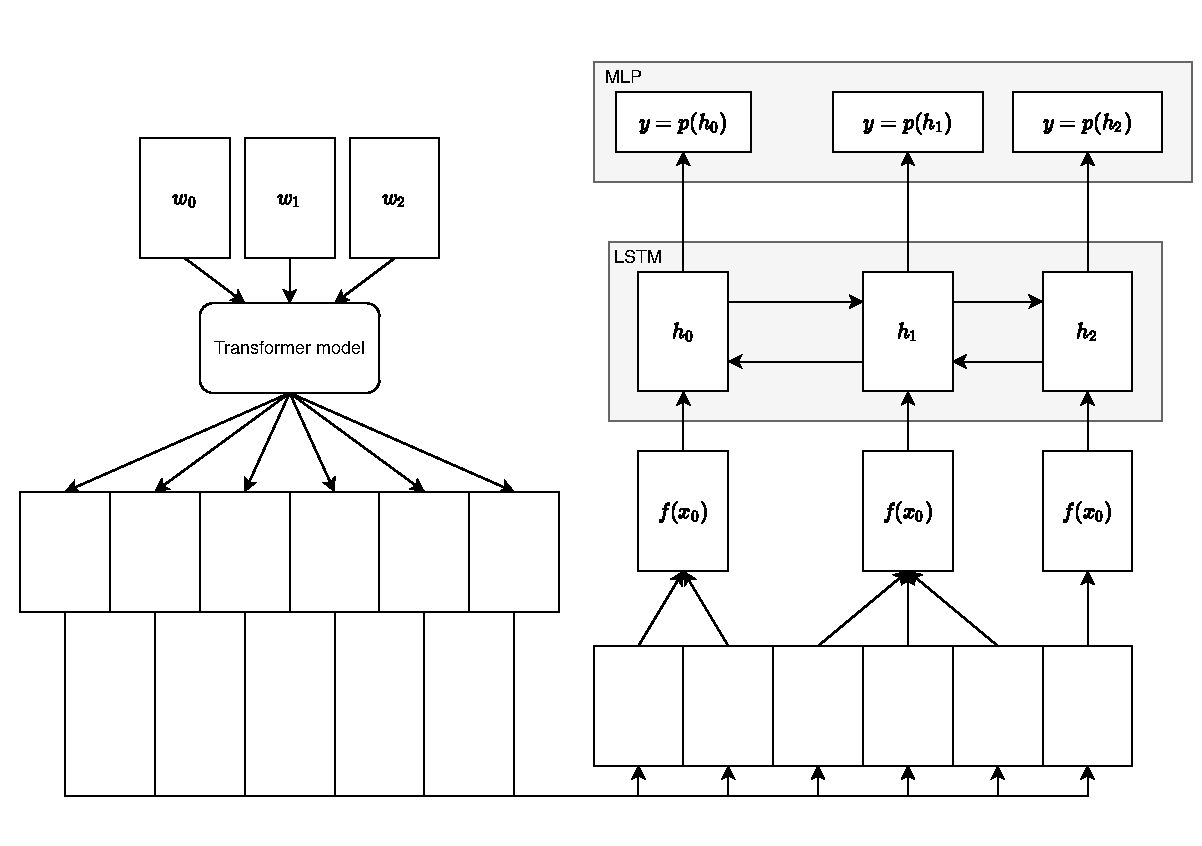
\includegraphics[scale=0.5]{model-outline.pdf}
		\caption{\label{fig:model} Procedure outline}
	\end{figure}
	
	\subsubsection{BPE features}b
        \label{sec:bpe-features}

             As mentioned previously, we look at methods for composing
     embeddings of BPE tokens into word embeddings. The XLMR model use
     12 layers to compute an embedding for a BPE token, and it has
     been shown in previous research
     \cite{kondratyukstraka,raganato2018analysis} [Find 1 or 2 more
     citations] that the different layers of the transformer model
     encode different types of information. To take advantage of this
     we compute BPE embeddings as a weighted sum of layer
     representations \cite{kondratyukstraka}.  That is, we initialize
     a parameter $w$ of dimension $l$, each from a normal distribution of mean $0$ and standard deviation $1$,
     where $l$ is the number of layers in the transformer model. If
     $r_{ji}$ is the layer representation at layer $j$ and token
     position $i$, we calculate the weighted sum as follows:
    \begin{equation}
		x_i = \sum_{1}^{J} softmax(w)_j r_{ji}
	\end{equation}

        Where $softmax(w)_j$ indicate the softmax of the learned
     importance of layer $j$. After we have computed a weighted sum for
     each BPE token we proceed to combine them into the tokens as they
     appear in the data.
    
            We look at three method in particular, summation and
     averaging along a dimension, and using an RNN. Summation and
     averaging have been used in previous work [CITATIONS], but using
     an RNN have not been explored before to our knowledge.
    
    	\paragraph{Sum:} For the sum method, we use an element-wise
     sum. That is, we take the sum for each dimension of the BPE
     embeddings separately. Thus, for token $i$ we calculate a
     composite embedding by summing over dimensions $1,\ldots,D$:
	
	\begin{equation}
	f(x)_i = \sum_{j=1}^{D} x_i^j
	\end{equation}
	

    	\paragraph{Mean:} In the mean method we calculate the sum and
     divide by the number of BPE embeddings in the word. Thus, for
     token $i$ we calculate a composite embedding by averaging over
     dimensions $1,\ldots,D$:
	
	\begin{equation}
	f(x)_{i} = \frac{1}{D}\sum_{j=1}^{D} x_i^j
	\end{equation}
	
	
	\paragraph{RNN:} For this method we employ a bidirectional LSTM
        to compose the BPE embeddings. For each multi-BPE
        token, we pass the sequence of BPE embeddings through an LSTM
        and use the final output as the word representation. 
    
	\subsubsection{Character features}
    	In addition to layer attention we use a character LSTM to
     extract a word representation based on characters. The final
     representation that we pass to the word-LSTM is the concatenation
     of the word representation based on BPE compositions and
     characters,
     $w_i = \text{concat}(f(bpe_0,...,bpe_K), f(c_0, ..., c_M))$
	
	\subsubsection{Label smoothing}
    	Given that many of the languages have a large number of
     morphological tags, we want to prevent the model from growing
     overconfident for certain classes. To address this issue we
     introduce label smoothing \cite{szegedy2016rethinking}, that is,
     instead of the incorrect classes having $0\%$ probability and the
     correct class $100\%$ probability we let each of the incorrect
     classes have a small probability.

        %The correct class is then assigned the probability $t$ by
     %$(1-\alpha)t + \alpha / |C|$ where $|C|$ is the number of
     %classes. \jp{I don't understand this formula (and I botched the
     %sentence trying to fix it :/ ... What is $t$? I was expecting
     %that you'd give the formula for the probability of the correct
     %class, but apparently I am mistaken.)}

     Let $\alpha$ be our smoothing value and $C$ the number of
     classes, then given a one-hot encoded target vector $t$ of size
     $C$, we calculate the smoothed probabilities as:
    \begin{equation}
        t_{smooth} = (1-\alpha)t + \frac{\alpha}{C}
    \end{equation}
    In words, we remove $\alpha$ from the correct class then
    distribute $\alpha$ uniformly among all classes.

     \subsection{Training}

    %\jp{add here a warning that we consider several possible training regimes}
	
     In our experiments we consider two possible training regimes. In
     the first regime we finetune the XLMR models parameters, in the
     second regime we only extract weights for BPE tokens, that is, we
     use the model as a feature extractor. In all cases, we use
     end-to-end training.
     
     When fine-tuning the model we freeze the XLMR parameters for the
     first epoch, (effectively not fine-tuning for the first epoch).
     When training the model we use cosine annealing learning rate
     with restarts every epoch, that is, the learning rate starts high
     then incrementally decreases to $1\mathrm{e}{-12}$ during $N$
     steps, where $N$ is the number of batches in an epoch. We use the
     Adam optimizer with a learning rate of $0.001$ for layer
     importance parameter ($w$ in \cref{sec:bpe-features}), the
     parameters of the word LSTM, classification layer, and BPE
     combination module (when an RNN is used). For the transformer
     parameters, we use a lower learning rate of $1\mathrm{e}{-06}$.

    %a_parser.add_argument('--xlmr_dropout', type=float, default=0.2) # number of input tokens changed to <unk>
    %a_parser.add_argument('--layer_dropout', type=float, default=0.1) # p that layer j is set to 0.
    %a_parser.add_argument('--layer_repr_dropout', type=float, default=0.4) # dropout for w (in all layers)
    %a_parser.add_argument('--transform_dropout', type=float, default=0.5) # dropout before predict(w)
    %a_parser.add_argument('--char_dropout', type=float, default=0.4) # dropout on w after char rnn
    %a_parser.add_argument('--bpe_dropout', type=float, default=0.4) # dropout on w after bpe composition
   
	\begin{table}%[h]
		\centering
		\begin{tabular}{lr}
			Parameter & Value \\
			\hline
			Epochs & 15 \\
			Batch size & 4 / 32 \\
			Character representation size & 128 \\
            Word LSTM size & 1536 \\
            Linear transform size & 1536 \\
			% optimizers
			Optimizer & Adam \\
			Learning rate & 0.001 \\
			Learning rate$_{xlmr}$ & 1e-06 \\
			% regularization
            Weight decay & 0.05 \\
			Label smoothing & 0.03 \\
            % described in text
            %Prediction dropout & 0.5 \\
			%Transformer dropout & 0.4 \\
            %Layer dropout & 0.1 \\
            %Input dropour & 0.2 \\
            %BPE dropout & 0.4 \\
            %Character dropout & 0.4 \\
		\end{tabular}
		\caption{\label{tab:parameters} Hyperparameters used for training the model. Slashed indicate the value of a parameter when we finetune or extract features.}
	\end{table}

        We use dropout throughout the model. We apply dropout on the
        input to the transformer, replacing 20 percent of the BPE tokens
        with \texttt{<UNK>}. After we have extracted layer features
        from the transformer we apply a dropout of $0.4$, and before
        computing the weighted sum of layers we apply full dropout on
        a layers with a probability of $0.1$. After the word LSTM have
        processed the sequence, but before the final prediction, we
        apply a dropout of $0.5$.

	
	\section{Results}
	\label{results}

        Even though our aim is to compare the relative performance of
        various BPE combination methods rather than to improve on the
        state of the art in absolute terms, we compare our results
        against the baseline reported by
        \citet{mccarthy2019sigmorphon}. This comparison serves the
        purpose of checking that our system is generally sound.  In
        particular, the actual state of the art, as reported by
        \citet{mccarthy2019sigmorphon}, use tree-bank concatenation,
        which means that results are not reported on a per-treebank
        basis.

    %
        The accuracy of our system computed by checking the prediction
        of morphological tags. We report in \cref{tab:results_tokens}
        the result for each of the three different methods, and the
        two training regimes.

	\begin{table} % [h]
	%\small
	\centering
	\begin{tabular}{l|c|ccc|ccc}
		& & \multicolumn{3}{c}{Finetuning} & \multicolumn{3}{c}{Feature extraction} \\
		Treebank & Baseline & Sum & Mean & RNN & Sum & Mean & RNN \\
		\hline
		% agglutinative languages
        Basque-BDT      & .676 & .905 & .906 & \textbf{.920} & .865 & .865 & \textbf{.888} \\
		Finnish-TDT     & .751 & .965 & .963 & \textbf{.967} & .930 & .931 & \textbf{.942} \\ 
		Turkish-IMST    & .620 & .898 & .891 & \textbf{.905} & .856 & .849 & \textbf{.866}\\
		Estonian-EDT    & .740 & .960 & .961 & \textbf{.962} & .931 & .934 & \textbf{.939} \\
		% fusional languages
		Spanish-AnCora  & .842 & .979 & .979 & \textbf{.980} & .968 & .967 & \textbf{.971} \\
		Arabic-PADT     & .770 & .952 & .953 & \textbf{.954} & .941 & .939 & \textbf{.948} \\
		Czech-CAC       & .771 & .976 & .976 & \textbf{.977} & .944 & .944 & \textbf{.952} \\
		Polish-LFG      & .657 & .959 & .956 & \textbf{.960} & .907 & .907 & \textbf{.928} \\
        \hline
        Average         & .728 & .949 & .948 & \textbf{.953} & .918 & .917 & \textbf{.929} \\
	\end{tabular}
	\caption{\label{tab:results_tokens} Accuracy for morphological tagging. We evaluate both when we finetune the XLMR model and when we only extract BPE embeddings.}
	\end{table}

        Our system performs better than the baseline. As a
     general trend we can see that the RNN method tends to perform
     better than the summation or averaging methods. This is
     consistent across both languages and training regimes, showing
     that while the changes are small, they are there consistenty.
    %
            Perhaps not surprisingly, we find that in general
     finetuning yields stronger performance than feature
     extraction. However, the difference is negligeble, increasing by
     $3.1$ percentage points for summation and averaging and $2.4$
     points for RNN.

     When finetuning we see the largest changes occur for Basque and
     Turkish, with an increased performance of $1.45$ points and $0.7$
     points when finetuning and using RNN over using mean or
     averaging. When only extracting features we see a larger
     increase when using an RNN, of $2.3$ points and $1.35$ points
     respectively.

	\begin{table}%[h]
	%\small
	\centering
	\begin{tabular}{l|c|ccc|ccc}
		& & \multicolumn{3}{c}{Finetuning} & \multicolumn{3}{c}{Feature extraction} \\
		Treebank & Baseline & Sum & Mean & RNN & Sum & Mean & RNN \\
		\hline
		Basque-BDT      & & .884 & .877 & \textbf{.901} & .789 & .780 & \textbf{.834} \\
		Finnish-TDT     & & .958 & .960 & \textbf{.965} & .856 & .847 & \textbf{.899} \\
		Turkish-IMST    & & .859 & .855 & \textbf{.884} & .741 & .735 & \textbf{.775} \\
		Estonian-EDT    & & .955 & 0 & 0 & .856 & .853 & \textbf{.901} \\
		Spanish-AnCora  & & 0 & 0 & 0 & .954 & .952 & \textbf{.962} \\
		Arabic-PADT     & & 0 & 0 & 0 & .923 & .902 & \textbf{.936} \\
		Czech-CAC       & & 0 & 0 & 0 & .887 & .881 & \textbf{.924} \\
		Polish-LFG      & & 0 & 0 & 0 & .844 & .840 & \textbf{.878} \\
        \hline
        Average         & .728 &  &  &  & .856 & .848 & \textbf{.888} \\
	\end{tabular}
	\caption{\label{tab:results_tokens_nochars} Without character LSTM, much more prominent changes in accuracy as expected.}
    \end{table}

    \Cref{tab:results_tokens} reports average accuracy for every word,
    thus also including those which are only composed of a single BPE
    token. To highlight the strengths and weaknesses of each
    composition method, we also compute the accuracy for tokens which
    are composed of two BPE tokens or more. The results can be seen in
    \cref{tab:results_large_tokens}.  We see again that RNN works
    better than summation or averaging BPE embeddings.

    
	\begin{table}%[h]
	%\small
	\centering
	\begin{tabular}{l|ccc|ccc}
		 & \multicolumn{3}{c}{Finetune} & \multicolumn{3}{c}{Feature extraction} \\
		Treebank & Sum & Mean & RNN & Sum & Mean & RNN  \\
		 \hline
		% agglutinative languages
        Basque-BDT      & .838 & .838 & \textbf{.863} & .802 & .803 & \textbf{.840} \\
		Finnish-TDT     & .950 & .947 & \textbf{.954} & .893 & .897 & \textbf{.913} \\ 
		Turkish-IMST    & .825 & .814 & \textbf{.846} & .807 & .796 & \textbf{.816} \\
		Estonian-EDT    & .946 & .957 & \textbf{.950} & .904 & .908 & \textbf{.916} \\
		% fusional languages
		Spanish-AnCora  & .964 & .963 & \textbf{.965} & .952 & .951 & \textbf{.959} \\
		Arabic-PADT     & .906 & .904 & \textbf{.913} & .927 & .925 & \textbf{.935}\\
		Czech-CAC       & .958 & .959 & \textbf{.962} & .915 & .916 & \textbf{.930} \\
		Polish-LFG      & .924 & .924 & \textbf{.933} & .834 & .833 & \textbf{.876} \\
        \hline
        Average         & .913 & .914 & \textbf{.923} & .891 & .878 & \textbf{.898} \\
	\end{tabular}
	\caption{\label{tab:results_large_tokens} Accuracy for morphological tagging on all tokens that are composed of 2 or more BPE tokens (with char-lstm).}
\end{table}

            We see the same trend for accuracy on tokens that are
     composed of two or more BPE tokens, as in the overall accuracy,
     where the RNN outperform both the sum and averaging methods. We
     can also see that the average increase in accuracy when using an
     RNN is larger. This holds for both when we only finetune the
     model and extract features.

    
    Given that the number of BPE tokens per natural-language token
     varies, we also look at the accuracy of the different methods
     given a different number of BPE tokens. We show per-language
     performance with the differnt methods in \cref{fig:bpe_lens}.

	\begin{figure}%[h!]
  	\centering
    \begin{tikzpicture} 
	\begin{axis}[
	name=,
	title={Finnish-TDT},
        xtick style={draw=none},
        ytick style={draw=none},
        xtick={1,2,3,3,4,5,6,7},
	typeset ticklabels with strut,
	legend pos=south west,
	ymajorgrids=false,
	grid style=dashed,
	height=5cm
	]
		\addplot[
		color=blue,
		mark=o,
                error bars/.cd, y dir=both, y explicit,
		]
		coordinates {
			(1, 0.978788725)
			(2, 0.954759661)
			(3, 0.951459606)
			(4, 0.920821114)
			(5, 0.959302326)
			(6, 0.953703704)
			(7, 0.95)
};
		\addplot[
		color=red,
		mark=o,
                error bars/.cd, y dir=both, y explicit,
		]
		coordinates {
			(1, 0.97711415)
			(2, 0.950989632)
			(3, 0.944331297)
			(4, 0.931573803)
			(5, 0.962209302)
			(6, 0.944444444)
			(7, 0.95)
};
		\addplot[
		color=green,
		mark=o,
                error bars/.cd, y dir=both, y explicit,
		]
		coordinates {
			(1, 0.978695693)
			(2, 0.956833176)
			(3, 0.954854039)
			(4, 0.929618768)
			(5, 0.962209302)
			(6, 0.962962963)
			(7, 0.975)
};
		\node[scale=0.5] at (1,-6) {10749};
		\node[scale=0.5] at (100,-6) {5305};
		\node[scale=0.5] at (200,-6) {2946};
		\node[scale=0.5] at (300,-6) {1023};
		\node[scale=0.5] at (400,-6) {344};
		\node[scale=0.5] at (500,-6) {108};
		\node[scale=0.5] at (600,-6) {40};

        \end{axis}
	\end{tikzpicture}
\begin{tikzpicture} 
	\begin{axis}[
	name=,
	title={Basque-BDT},
        xtick style={draw=none},
        ytick style={draw=none},
        xtick={1,2,3,3,4,5,6,7},
	typeset ticklabels with strut,
	legend pos=south west,
	ymajorgrids=false,
	grid style=dashed,
	height=5cm
	]
		\addplot[
		color=blue,
		mark=o,
                error bars/.cd, y dir=both, y explicit,
		]
		coordinates {
			(1, 0.955423477)
			(2, 0.860581432)
			(3, 0.811436351)
			(4, 0.768831169)
			(5, 0.746666667)
			(6, 0.833333333)
			(7, 1.0)
};
		\addplot[
		color=red,
		mark=o,
                error bars/.cd, y dir=both, y explicit,
		]
		coordinates {
			(1, 0.957800892)
			(2, 0.865582995)
			(3, 0.803948264)
			(4, 0.755844156)
			(5, 0.693333333)
			(6, 0.916666667)
			(7, 1.0)
};
		\addplot[
		color=green,
		mark=o,
                error bars/.cd, y dir=both, y explicit,
		]
		coordinates {
			(1, 0.962109955)
			(2, 0.889340419)
			(3, 0.827093261)
			(4, 0.8)
			(5, 0.76)
			(6, 1.0)
			(7, 1.0)
};
		\node[scale=0.5] at (1,-6) {6730};
		\node[scale=0.5] at (100,-6) {3199};
		\node[scale=0.5] at (200,-6) {1469};
		\node[scale=0.5] at (300,-6) {385};
		\node[scale=0.5] at (400,-6) {75};
		\node[scale=0.5] at (500,-6) {12};
		\node[scale=0.5] at (600,-6) {5};

        \end{axis}
	\end{tikzpicture}
\begin{tikzpicture} 
	\begin{axis}[
	name=,
	title={Turkish-IMST},
        xtick style={draw=none},
        ytick style={draw=none},
        xtick={1,2,3,3,4,5,6,7},
	typeset ticklabels with strut,
	legend pos=south west,
	ymajorgrids=false,
	grid style=dashed,
	height=5cm
	]
		\addplot[
		color=blue,
		mark=o,
                error bars/.cd, y dir=both, y explicit,
		]
		coordinates {
			(1, 0.943162147)
			(2, 0.849106552)
			(3, 0.756457565)
			(4, 0.819767442)
			(5, 0.913043478)
			(6, 0.769230769)
			(7, 0.75)
};
		\addplot[
		color=red,
		mark=o,
                error bars/.cd, y dir=both, y explicit,
		]
		coordinates {
			(1, 0.939122908)
			(2, 0.841826605)
			(3, 0.745387454)
			(4, 0.802325581)
			(5, 0.739130435)
			(6, 0.692307692)
			(7, 1.0)
};
		\addplot[
		color=green,
		mark=o,
                error bars/.cd, y dir=both, y explicit,
		]
		coordinates {
			(1, 0.94287363)
			(2, 0.870946393)
			(3, 0.776752768)
			(4, 0.843023256)
			(5, 0.869565217)
			(6, 0.846153846)
			(7, 0.75)
};
		\node[scale=0.5] at (1,-6) {3466};
		\node[scale=0.5] at (100,-6) {1511};
		\node[scale=0.5] at (200,-6) {542};
		\node[scale=0.5] at (300,-6) {172};
		\node[scale=0.5] at (400,-6) {23};
		\node[scale=0.5] at (500,-6) {13};
		\node[scale=0.5] at (600,-6) {4};

        \end{axis}
	\end{tikzpicture}
\begin{tikzpicture} 
	\begin{axis}[
	name=,
	title={Estonian-EDT},
        xtick style={draw=none},
        ytick style={draw=none},
        xtick={1,2,3,3,4,5,6,7},
	typeset ticklabels with strut,
	legend pos=south west,
	ymajorgrids=false,
	grid style=dashed,
	height=5cm
	]
		\addplot[
		color=blue,
		mark=o,
                error bars/.cd, y dir=both, y explicit,
		]
		coordinates {
			(1, 0.970751181)
			(2, 0.948556876)
			(3, 0.94276436)
			(4, 0.938250429)
			(5, 0.962831858)
			(6, 0.940789474)
			(7, 0.946808511)
};
		\addplot[
		color=red,
		mark=o,
                error bars/.cd, y dir=both, y explicit,
		]
		coordinates {
			(1, 0.970914127)
			(2, 0.94991511)
			(3, 0.942967323)
			(4, 0.939965695)
			(5, 0.957522124)
			(6, 0.947368421)
			(7, 0.946808511)
};
		\addplot[
		color=green,
		mark=o,
                error bars/.cd, y dir=both, y explicit,
		]
		coordinates {
			(1, 0.970791918)
			(2, 0.951952462)
			(3, 0.945605845)
			(4, 0.947398513)
			(5, 0.968141593)
			(6, 0.947368421)
			(7, 0.936170213)
};
		\node[scale=0.5] at (1,-6) {24548};
		\node[scale=0.5] at (100,-6) {11780};
		\node[scale=0.5] at (200,-6) {4927};
		\node[scale=0.5] at (300,-6) {1749};
		\node[scale=0.5] at (400,-6) {565};
		\node[scale=0.5] at (500,-6) {152};
		\node[scale=0.5] at (600,-6) {94};

        \end{axis}
	\end{tikzpicture}
\begin{tikzpicture} 
	\begin{axis}[
	name=,
	title={Arabic-PADT},
        xtick style={draw=none},
        ytick style={draw=none},
        xtick={1,2,3,3,4,5,6,7},
	typeset ticklabels with strut,
	legend pos=south west,
	ymajorgrids=false,
	grid style=dashed,
	height=5cm
	]
		\addplot[
		color=blue,
		mark=o,
                error bars/.cd, y dir=both, y explicit,
		]
		coordinates {
			(1, 0.967134623)
			(2, 0.912252325)
			(3, 0.892663712)
			(4, 0.883268482)
			(5, 0.866666667)
};
		\addplot[
		color=red,
		mark=o,
                error bars/.cd, y dir=both, y explicit,
		]
		coordinates {
			(1, 0.968529193)
			(2, 0.909017388)
			(3, 0.893648449)
			(4, 0.898832685)
			(5, 0.933333333)
};
		\addplot[
		color=green,
		mark=o,
                error bars/.cd, y dir=both, y explicit,
		]
		coordinates {
			(1, 0.967971365)
			(2, 0.91589163)
			(3, 0.907434761)
			(4, 0.906614786)
			(5, 0.933333333)
};
		\node[scale=0.5] at (1,-6) {21512};
		\node[scale=0.5] at (100,-6) {4946};
		\node[scale=0.5] at (200,-6) {2031};
		\node[scale=0.5] at (300,-6) {257};
		\node[scale=0.5] at (400,-6) {15};

        \end{axis}
	\end{tikzpicture}
\begin{tikzpicture} 
	\begin{axis}[
	name=,
	title={Spanish-ANCORA},
        xtick style={draw=none},
        ytick style={draw=none},
        xtick={1,2,3,3,4,5,6,7},
	typeset ticklabels with strut,
	legend pos=south west,
	ymajorgrids=false,
	grid style=dashed,
	height=5cm
	]
		\addplot[
		color=blue,
		mark=o,
                error bars/.cd, y dir=both, y explicit,
		]
		coordinates {
			(1, 0.983232268)
			(2, 0.967484739)
			(3, 0.958818636)
			(4, 0.937984496)
			(5, 0.905660377)
			(6, 0.92)
			(7, 0.75)
};
		\addplot[
		color=red,
		mark=o,
                error bars/.cd, y dir=both, y explicit,
		]
		coordinates {
			(1, 0.982910695)
			(2, 0.966986421)
			(3, 0.956738769)
			(4, 0.935400517)
			(5, 0.905660377)
			(6, 0.92)
			(7, 0.75)
};
		\addplot[
		color=green,
		mark=o,
                error bars/.cd, y dir=both, y explicit,
		]
		coordinates {
			(1, 0.983416024)
			(2, 0.968730534)
			(3, 0.956322795)
			(4, 0.937984496)
			(5, 0.943396226)
			(6, 0.92)
			(7, 0.75)
};
		\node[scale=0.5] at (1,-6) {43536};
		\node[scale=0.5] at (100,-6) {8027};
		\node[scale=0.5] at (200,-6) {2404};
		\node[scale=0.5] at (300,-6) {387};
		\node[scale=0.5] at (400,-6) {53};
		\node[scale=0.5] at (500,-6) {25};
		\node[scale=0.5] at (600,-6) {4};

        \end{axis}
	\end{tikzpicture}
\begin{tikzpicture} 
	\begin{axis}[
	name=,
	title={Polish-LFG},
        xtick style={draw=none},
        ytick style={draw=none},
        xtick={1,2,3,3,4,5,6,7},
	typeset ticklabels with strut,
	legend pos=south west,
	ymajorgrids=false,
	grid style=dashed,
	height=5cm
	]
		\addplot[
		color=blue,
		mark=o,
                error bars/.cd, y dir=both, y explicit,
		]
		coordinates {
			(1, 0.976847521)
			(2, 0.934393638)
			(3, 0.913963329)
			(4, 0.902439024)
			(5, 0.894736842)
			(6, 0.888888889)
};
		\addplot[
		color=red,
		mark=o,
                error bars/.cd, y dir=both, y explicit,
		]
		coordinates {
			(1, 0.972754911)
			(2, 0.930815109)
			(3, 0.921015515)
			(4, 0.912601626)
			(5, 0.855263158)
			(6, 0.888888889)
};
		\addplot[
		color=green,
		mark=o,
                error bars/.cd, y dir=both, y explicit,
		]
		coordinates {
			(1, 0.974158092)
			(2, 0.943936382)
			(3, 0.921720733)
			(4, 0.916666667)
			(5, 0.881578947)
			(6, 0.888888889)
};
		\node[scale=0.5] at (1,-6) {8552};
		\node[scale=0.5] at (100,-6) {2515};
		\node[scale=0.5] at (200,-6) {1418};
		\node[scale=0.5] at (300,-6) {492};
		\node[scale=0.5] at (400,-6) {76};
		\node[scale=0.5] at (500,-6) {9};

        \end{axis}
	\end{tikzpicture}
\begin{tikzpicture} 
	\begin{axis}[
	name=,
	title={Czech-CAC},
        xtick style={draw=none},
        ytick style={draw=none},
        xtick={1,2,3,3,4,5,6,7},
	typeset ticklabels with strut,
	legend pos=south west,
	ymajorgrids=false,
	grid style=dashed,
	height=5cm
	]
		\addplot[
		color=blue,
		mark=o,
                error bars/.cd, y dir=both, y explicit,
		]
		coordinates {
			(1, 0.987536707)
			(2, 0.963371471)
			(3, 0.949902981)
			(4, 0.958403598)
			(5, 0.905084746)
			(6, 0.957446809)
			(7, 1.0)
};
		\addplot[
		color=red,
		mark=o,
                error bars/.cd, y dir=both, y explicit,
		]
		coordinates {
			(1, 0.987809875)
			(2, 0.963618405)
			(3, 0.950608573)
			(4, 0.960089938)
			(5, 0.901694915)
			(6, 0.957446809)
			(7, 1.0)
};
		\addplot[
		color=green,
		mark=o,
                error bars/.cd, y dir=both, y explicit,
		]
		coordinates {
			(1, 0.987400123)
			(2, 0.967240102)
			(3, 0.953254542)
			(4, 0.960089938)
			(5, 0.898305085)
			(6, 0.957446809)
			(7, 1.0)
};
		\node[scale=0.5] at (1,-6) {29286};
		\node[scale=0.5] at (100,-6) {12149};
		\node[scale=0.5] at (200,-6) {5669};
		\node[scale=0.5] at (300,-6) {1779};
		\node[scale=0.5] at (400,-6) {295};
		\node[scale=0.5] at (500,-6) {47};
		\node[scale=0.5] at (600,-6) {3};

        \end{axis}
	\end{tikzpicture}

                \caption{\label{fig:bpe_lens} Per-language accuracy on
     tokens with different number of BPE components. Values of seven
     of the $x$-axis also include all tokens who are composed of seven
     or more BPE tokens. We indicate the method by encoding summation
     as blue, averaging as red and RNN as green. The accuracy is given
     on the $y$-axis. The number above the $x$-axis indicate the
     support for the result, i.e. how many samples the accuracy was
     calculated on. The confidence interval is calculated using the
     Agresti-Coull interval.}
		%\caption{\label{fig:bpe_lens} Per language accuracy of
        %          tokens composed of more than two BPE tokens\jp{it is
        %            the case that the methods always coincide at 1
        %            token? Either say so, or this graph could also
        %            include this data. }. The x-axis indicates how
        %          many BPE tokens a word is composed of; and the
        %          y-axis shows the accuracy. The different methods are
        %          distinguished by color, where blue is the summation
        %          method, red the mean and green RNN. \jp{? The number
        %            of samples for 6-bpe token is probably low and not
        %            that ``accurate''. Perhaps you could show (indicative) error
        %            bars? https://en.wikipedia.org/wiki/Binomial_proportion_confidence_interval}}
	\end{figure}

	
	
	\section{Discussion}

        \subsection{BPE composition methods}
        Analogously to character embeddings, the RNN method seem to
        provide stronger results than using either Sum or Mean for
        combining BPE tokens. We conjecture that this discrepancy is
        can be attributed to the commutativity of the Sum and Mean
        operations. That is, the ordering of elements within a word
        does not affect the result of applying Sum or Mean.

              Intuitively, when using the Sum or Mean method the
     system won't be aware of, for example, split affixes. For example
     if the word "derivable" is split into ``deriv'' + ``ab'' + ``le''
     the system won't be aware that ``able'' is a meaningful unit in
     terms of morphology (and by extension, semantics).

        %\jp{In particular, the position of an affix is lost if the
     %word which includes it is split in several tokens.}
        
    (len1 about the same for all languages)

    \subsection{Language typology}
    With regards to the performance of the different methods for
     different language typologies we see in [main-results, figure]
     that the gap between the RNN methods and the Sum and Mean method
     is larger. This is expecially prominent in \cref{fig:bpe_lens}
     where the green line is above the red and blue for most lengths.

    

    
    \section{Conclusions}
    	As a general summary of our work, we highlight that language typology is not irrelevant when working with models that employ byte-pair encoding.
	
	%\section*{Acknowledgments}
	
	
	% include your own bib file like this:
	\bibliographystyle{coling}
	\bibliography{coling2020}
	
\end{document}
